\section{Introduction}

Ti-89 is a graphing calculator released by Texas Instruments. Originally, there was a model called TI-92, but it was considered a computer rather than a calculator because it had a QWERTY keyboard, and the TI-89 was an improved model to bring it to the test of the College Board. TI-89 Titanium is a sequel based on TI-92 Voyage 200. (From Wikipedia)


\begin{figure}[htbp]
    \centering
    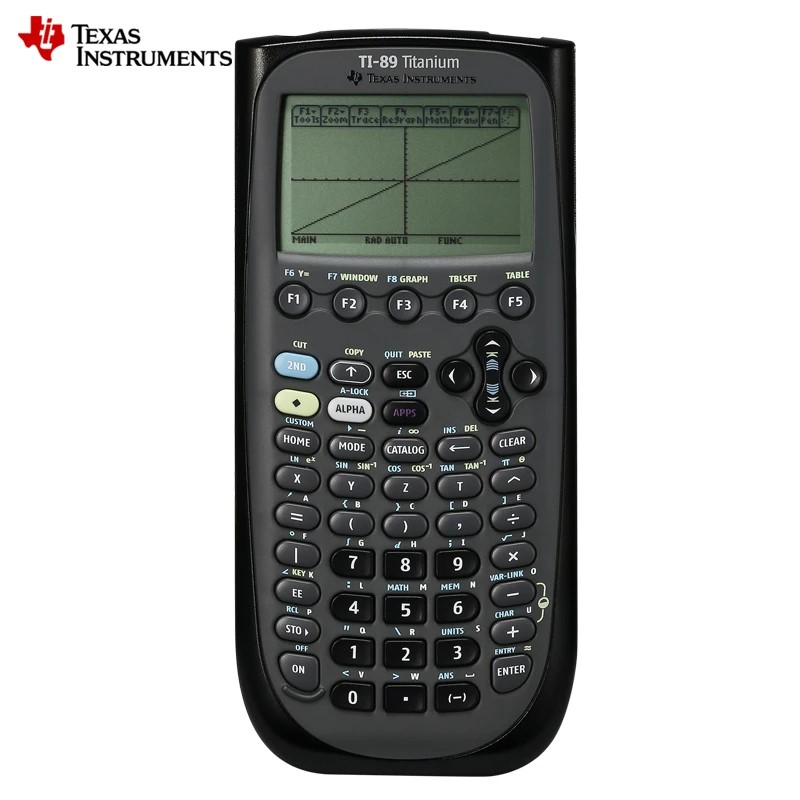
\includegraphics[height=10cm]{images/Ti-89_Titanium.jpg}
    \label{Ti-89_Titanium}
\end{figure}

\noindent For further references, see \href{https://education.ti.com/en}{Texas Industry}. Also, you can download instructions at \href{https://education.ti.com/en/guidebook/details/en/FA1DC891957E4700B46A67255850C592/89ti}{Instruction}

The writer of this document is Dohyun Nam, and I made this document because the original instruction was too long and it had too much unnecessary information. I got to use this calculator because of AP exams, such as Calculus BC, Statistics, Physics C: Mechanics, etc. There are a few main functions that I use, and I wanted to organize them so that I don't have to search from the original document. That's why I made this document, and it has some mathematical principles within, so I got to check my mathematical logic. 